\section{Mixing and Decay of the \texorpdfstring{\BsBsbar{}}{Bs0Bs0bar} System}
\label{sec:pheno_mix}

%%%%%%%%%%%%%%%%%%%%%%%%%
\subsection{Mixing}
\label{sec:pheno_mix_mix}
%%%%%%%%%%%%%%%%%%%%%%%%%

A meson produced in a pure $\Bs$ or $\Bsbar$ state will evolve in time and become a mixture of these two flavour states. If the time
coordinate in the \BsBsbar{} centre-of-mass system is given by $t$, the state of the system ($\Psi$) can be written as
\begin{equation}
  \label{eq:timeEvolBBbarState}
  |\Psi(t)\rangle = a(t)\,\Bsst + b(t)\,\Bsbarst
  \ .
\end{equation}
The states $\Bsst\equiv|\text{s}\bar{\text{b}}\rangle$ and $\Bsbarst\equiv|\bar{\text{s}}\text{b}\rangle$ are the \emph{flavour
eigenstates} of the system and $a$ and $b$ are coefficients that describe its time dependence.

Assuming that the time scale of interest is much larger than the time scale of strong interactions, the Weisskopf-Wigner approximation can
be used and the decay of the system has an exponential time dependence~\cite{Weisskopf:1930au,*Weisskopf:1930ps,*Lee:1957qq}. The time
evolution then follows from a Schr\"odinger equation with a constant Hamiltonian, which is given by\footnote{All equations in this chapter
are expressed in \emph{natural units}, in which the reduced Planck constant and the speed of light are equal to one ($\hbar \equiv c \equiv
1$).}
\begin{equation}
  \label{eq:timeEvolSchr}
  i\; \frac{\partial}{\partial t} \begin{pmatrix} a(t) \\ b(t) \end{pmatrix}
    = \vec{H} \begin{pmatrix} a(t) \\ b(t) \end{pmatrix}
    \ .
\end{equation}

Without loss of generality, the Hamiltonian matrix $\vec{H}$ can be written as the sum of a Hermitian matrix and an anti-Hermitian matrix:
$\vec{H} \equiv \vec{M} - \tfrac{i}{2}\,\vec{\Gamma}$, where the \emph{mass matrix} $\vec{M}$ and the \emph{decay matrix} $\vec{\Gamma}$
are both Hermitian. Assuming CPT invariance, the mass and lifetime of a particle are equal to the respective mass and lifetime of the
corresponding anti-particle. This results in equal diagonal elements of both the mass and decay matrices:
\begin{equation}
  \label{eq:timeEvolHamil}
  \vec{H}
    \equiv \begin{pmatrix} H_0 & H_{12} \\ H_{21} & H_0 \end{pmatrix}
    = \vec{M} - \tfrac{i}{2}\,\vec{\Gamma}
    \equiv \begin{pmatrix} \ms & \mmix \\ \mmix^* & \ms \end{pmatrix}
      - \tfrac{i}{2} \begin{pmatrix} \Gs & \gmix \\ \gmix^* & \Gs \end{pmatrix}
    \ ,
\end{equation}
where $\ms$ is the $\Bs$ mass and $\Gs$ the $\Bs$ decay width.

Mixing of the $\Bs$ and $\Bsbar$ states is governed by the off-diagonal elements of the Hamiltonian. The parameter $\mmix$ is the
\emph{dispersive} part of $H_{12}$. This part originates from contributions of virtual intermediate states to the mixing process and is
dominated by the diagrams with virtual top quarks (Figure~\ref{fig:mixing} on page~\pageref{fig:mixing}). $\gmix$ is the \emph{absorptive}
part, which originates from contributions of real states into which both $\Bs$ and $\Bsbar$ can decay.

The absorptive part of the mixing process is dominated by tree-level $\btoccs$ transitions~\cite{Lenz:2006hd,*Lenz:2011ti} and, therefore,
effects of physics beyond the Standard Model in $\gmix$ are expected to be small. The virtual process that dominates $\mmix$, on the other
hand, can be affected significantly and may lead to a deviation in the phase $\phis$.

To solve Equation~\ref{eq:timeEvolSchr} and obtain expressions for the time evolution of the $\Bs$ and $\Bsbar$ states, the system is
decoupled with a transformation of the flavour eigenstates that diagonalizes the Hamiltonian matrix. The decoupled states are \emph{mass
eigenstates}, which have definite mass and lifetime. With transformation matrix $\vec{P}$, diagonalized Hamiltonian $\vec{H'}$ and
mass-eigenstate coefficients $a'$ and $b'$, the transformation is specified by
\begin{equation}
  \label{eq:timeEvolTrans}
  \vec{H'} = \vec{P}^{-1}\,\vec{H}\,\vec{P}
  \qquad \text{and} \qquad
  \begin{pmatrix} a(t) \\ b(t) \end{pmatrix}
    = \vec{P}\, \begin{pmatrix} a'(t) \\ b'(t) \end{pmatrix}
  \ .
\end{equation}
The two eigenvalues of $\vec{H}$ become the diagonal elements of the decoupled Hamiltonian $\vec{H'}$ and the transformation matrix is
constructed from the corresponding eigenvectors:
\begin{subequations}
  \label{eq:timeEvolMassStates}
  \begin{align}
    \vec{H'} &\equiv \begin{pmatrix} \mL & 0 \\ 0 & \mH \end{pmatrix}
             - \tfrac{i}{2}\, \begin{pmatrix} \GL & 0 \\ 0 & \GH \end{pmatrix}
    \label{eq:timeEvolMassStatesHamil1} \\
    &= \begin{pmatrix} H_0 - \sqrt{H_{12} H_{21}} & 0 \\ 0 & H_0 + \sqrt{H_{12} H_{21}} \end{pmatrix}
    \label{eq:timeEvolMassStatesHamil2} \\
    \vec{P}  &= \begin{pmatrix*}[r]
                   \alpha\sqrt{H_{12}} &  \beta\sqrt{H_{12}} \\
                  -\alpha\sqrt{H_{21}} & +\beta\sqrt{H_{21}}
                \end{pmatrix*}
    \label{eq:timeEvolMassTrans}
    \ ,
  \end{align}
\end{subequations}
where the subscript L (light) is used for the state with the smaller mass and the subscript H (heavy) for the state with the larger mass.
The parameters $\alpha$ and $\beta$ are arbitrary constants as far as diagonalizing the Hamiltonian is concerned.

Mass and decay parameters of $\Bs$ and $\Bsbar$ are related to the masses and decay widths of $\BL$ and $\BH$ by
Equations~\ref{eq:timeEvolMassStatesHamil1} and \ref{eq:timeEvolMassStatesHamil2}: $H_0 = \tfrac{1}{2}\,(\mH+\mL) -
\tfrac{i}{4}\,(\GL+\GH)$ and $\sqrt{H_{12} H_{21}} = \tfrac{1}{2}\,(\mH-\mL) + \tfrac{i}{4}\,(\GL-\GH)$. Using also
Equation~\ref{eq:timeEvolHamil}:
\begin{subequations}
  \label{eq:DmsDGsDef}
  \begin{alignat}{2}
    \ms   &\,=\,&     \Re(H_0) &\,=\, \tfrac{1}{2}\,(\mH+\mL)     \\
    \Gs &\,=\,& -2\,\Im(H_0) &\,=\, \tfrac{1}{2}\,(\GL+\GH)
  \end{alignat}%
  \begin{align}
    \Dms   &\equiv \mH-\mL = 2\,\Re\!\left(\!\sqrt{H_{12} H_{21}}\right) \nonumber\\
             &= 2\,\Re\!\left(\sqrt{(\mmix-\tfrac{i}{2}\,\gmix)\,(\mmix^*-\tfrac{i}{2}\,\gmix^*)}\right) \\
    \DGs &\equiv \GL-\GH = 4\,\Im\!\left(\!\sqrt{H_{12} H_{21}}\right) \nonumber\\
             &= 4\,\Im\!\left(\sqrt{(\mmix-\tfrac{i}{2}\,\gmix)\,(\mmix^*-\tfrac{i}{2}\,\gmix^*)}\right)
  \end{align}
\end{subequations}
With these definitions of $\Dms$ and $\DGs$, the expression for $\sqrt{H_{12} H_{21}}$ reads
\begin{equation}
  \label{eq:HHmixSq}
  \begin{gathered}
    \sqrt{H_{12} H_{21}} = \sqrt{(\mmix-\tfrac{i}{2}\,\gmix)\,(\mmix^*-\tfrac{i}{2}\,\gmix^*)}
                          = \tfrac{1}{2}\,\Dms + \tfrac{i}{4}\,\DGs \\
    4\,|\mmix|^2 - |\gmix|^2 - 4i\,\Re(\mmix\,\gmix^*) = \Dms^2 - \tfrac{1}{4}\,\DGs^2 + i\,\Dms\,\DGs \ ,
  \end{gathered}
\end{equation}
which yields the relations
\begin{subequations}
  \label{eq:DmsDGsMmixGmix}
  \begin{align}
    \label{eq:DmsDGsMmixGmix_1}
    \Dms^2 - \tfrac{1}{4}\,\DGs^2 &= 4\,|\mmix|^2 - |\gmix|^2 \\[0.5em]
    \label{eq:DmsDGsMmixGmix_2}
    \Dms\,\DGs &= -4\,\Re(\mmix\,\gmix^*) = 4\,|\mmix|\,|\gmix|\,\cos\phimix \ ,
  \end{align}
\end{subequations}
where the parameter $\phimix$ is defined as the phase difference between $\mmix$ and $\gmix$:
$\phimix\text{\textequiv}\arg\big(\text{--}\frac{\mmix}{\gmix}\big)$.

To find the transformation between flavour eigenstates and mass eigenstates, the state of Equation~\ref{eq:timeEvolBBbarState} is expressed
in matrix form and the transformation of Equation~\ref{eq:timeEvolTrans} is applied:
\begin{equation}
  \label{eq:timeEvolBLBHState}
  \begin{split}
    |\Psi(t)\rangle &= \begin{pmatrix} a'(t) & b'(t) \end{pmatrix} \begin{pmatrix} \BLst \\ \BHst \end{pmatrix} \\
                    &= \begin{pmatrix} a(t) & b(t) \end{pmatrix} \begin{pmatrix} \Bsst \\ \Bsbarst \end{pmatrix}
                     = \begin{pmatrix} a'(t) & b'(t) \end{pmatrix} \vec{P}^\text{T} \begin{pmatrix} \Bsst \\ \Bsbarst \end{pmatrix}
    \ .
  \end{split}
\end{equation}
By comparing the first and second line of Equation~\ref{eq:timeEvolBLBHState} it can be seen that the transformation matrix between flavour
eigenstates and mass eigenstates is the transpose of the matrix that diagonalizes the Hamiltonian (Equation~\ref{eq:timeEvolMassTrans}).

Introducing the complex parameters $p$ and $q$ and normalizing the mass eigenstates, the transformation to flavour eigenstates can be
expressed as
% fix a phase convention?
\begin{equation}
  \label{eq:timeEvolTransInv}
  \begin{pmatrix} \BLst \\ \BHst \end{pmatrix}
    = \vec{P}^\text{T} \begin{pmatrix} \Bsst \\ \Bsbarst \end{pmatrix}
    = \begin{pmatrix} p & +q \\ p & -q \end{pmatrix}
      \begin{pmatrix} \Bsst \\ \Bsbarst \end{pmatrix}
  \qquad
  \text{with } |p|^2+|q|^2\equiv1
  \ .
\end{equation}
From Equations~\ref{eq:timeEvolMassTrans} and \ref{eq:timeEvolTransInv} it now follows that $\alpha=\beta$ and, also with
Equation~\ref{eq:timeEvolHamil},
\begin{equation}
  \label{eq:qpDef}
  \qp = -\sqrt{\frac{H_{21}}{H_{12}}} = -\sqrt{\frac{\mmix^*-\tfrac{i}{2}\,\gmix^*}{\mmix-\tfrac{i}{2}\,\gmix}}
  \quad .
\end{equation}

The time evolution of the mass eigenstates is obtained by solving the Schr\"o\-ding\-er equation with the diagonal Hamiltonian of
Equation~\ref{eq:timeEvolMassStates}, which gives decoupled exponential decays for $\BL$ and $\BH$. Transforming back to the flavour
basis then gives the coupled time evolution of $\Bs$ and $\Bsbar$:
\begin{subequations}
  \label{eq:timeEvolTimeCoefs}
  \begin{equation}
    \begin{split}
      \begin{pmatrix} a(t) \\ b(t) \end{pmatrix}
        &= e^{-i\,\vec{H}\,t} \begin{pmatrix} a(0) \\ b(0) \end{pmatrix} \\
        &= \vec{P} \begin{pmatrix} a'(t) \\ b'(t) \end{pmatrix}
         = \vec{P}\, e^{-i\,\vec{H'}\,t} \begin{pmatrix} a'(0) \\ b'(0) \end{pmatrix}
         = \vec{P}\, e^{-i\,\vec{H'}\,t}\, \vec{P}^{-1} \begin{pmatrix} a(0) \\ b(0) \end{pmatrix}
    \end{split}
  \end{equation}%
  \begin{align}
    e^{-i\,\vec{H}\,t} &= \vec{P}\, e^{-i\,\vec{H'}\,t}\, \vec{P}^{-1} \nonumber\\
                       &= \begin{pmatrix*}[r] p & p \\ q & -q \end{pmatrix*}\!
                          \begin{pmatrix} e^{-i\,(\mL-i\,\GL/2)\,t} & 0 \\ 0 & e^{-i\,(\mH-i\,\GH/2)\,t} \end{pmatrix}\!
                          \begin{pmatrix*}[r] q & p \\ q & -p \end{pmatrix*} \frac{1}{2\,p\,q} \nonumber\\
                       &= \begin{pmatrix*}[r] g_+(t) & \pq\,g_-(t) \\ \qp\,g_-(t) & g_+(t) \end{pmatrix*}
    \ ,
  \end{align}
\end{subequations}
where the functions $g_\pm$ are given by
\begin{align}
  \label{eq:timeEvolQp}
  g_\pm(t) &\equiv \tfrac{1}{2}\, \left( e^{-i\,(\mL-i\,\GL/2)\,t} \pm e^{-i\,(\mH-i\,\GH/2)\,t} \right) \\
           &= \tfrac{1}{2}\, e^{-i\,\ms\,t}\, e^{-\Gs/2\,t}
                \left( e^{+i\,\Dms/2\,t}\, e^{-\DGs/4\,t} \pm e^{-i\,\Dms/2\,t}\, e^{+\DGs/4\,t} \right) \nonumber
           \ .
\end{align}

The time evolution for mesons produced as $\Bs$ ($a(0)=1$ and $b(0)=0$) and mesons produced as $\Bsbar$ ($a(0)=0$ and $b(0)=1$) can now be
inferred from Equations~\ref{eq:timeEvolBBbarState} and \ref{eq:timeEvolTimeCoefs}:
\begin{subequations}
  \label{eq:timeEvolBBbarStateInit}
  \begin{align}
    |\Psi_{\Bs}(t)\rangle    = g_+(t)\,\Bsst    + \qp\,g_-(t)\,\Bsbarst \\
    |\Psi_{\Bsbar}(t)\rangle = g_+(t)\,\Bsbarst + \pq\,g_-(t)\,\Bsst
  \end{align}
\end{subequations}

%%%%%%%%%%%%%%%%%%%%%%%%%%%%%
\subsection{Mixing and Decay}
\label{sec:pheno_mix_decay}
%%%%%%%%%%%%%%%%%%%%%%%%%%%%%

Time-dependent amplitudes for mixing and decay of the \BsBsbar{} system are obtained by combining the state of
Equation~\ref{eq:timeEvolBBbarState} with the amplitudes for the decays of $\Bsst$ and $\Bsbarst$. Assuming the system is produced as
either $\Bsst$ or $\Bsbarst$, the required time-dependent states are given by Equation~\ref{eq:timeEvolBBbarStateInit}. The decay amplitude
of a decay of $\Bsst$ into a final state $\fst$ is labelled by $\Af$. The amplitude for a system produced as a $\Bs$, being in a $\Bs$
state at the time of decay and decaying into $\fst$ is given by $\langle\Bs|\Psi_{\Bs}(t)\rangle\,\Af \propto g_+(t)\,\Af$.

If also $\Bsbarst$ can decay into the final state there is a second contribution to the $\Bstof$ process, which is proportional to the
decay amplitude labelled by $\Abarf$. Also considering decays into the CP conjugate of the final state, $\fbarst$, the amplitudes of the
four possible combinations of initial and final states are given by
\begin{equation}
  \label{eq:mixDecayAmps}
  \begin{alignedat}{4}
    \mathcal{A}(\Bstof) &\propto& & g_+\, \Af + \qp\, g_-\, \Abarf &
    \quad
    \mathcal{A}(\Bstofbar) &\propto& \;\qp \Big( & g_-\, \Abarfbar + \pq\, g_+\, \Afbar \Big)
    \\
    \mathcal{A}(\Bsbartof) &\propto& \;\pq \Big( & g_-\, \Af + \qp\, g_+\, \Abarf \Big) &
    \mathcal{A}(\Bsbartofbar) &\propto& & g_+\, \Abarfbar + \pq\, g_-\, \Afbar
    \ .
  \end{alignedat}
\end{equation}

Notice that the amplitudes for the processes with final state $\fbarst$ have the same structure as the amplitudes for the processes with
final state $\fst$. $\mathcal{A}(\Bsbartofbar)$ and $\mathcal{A}(\Bstofbar)$ can be obtained from $\mathcal{A}(\Bstof)$ and
$\mathcal{A}(\Bsbartof)$, respectively, by interchanging $p$ and $q$, replacing $\Af$ by $\Abarfbar$ and replacing $\Abarf$ by $\Afbar$.
The amplitude for $\Bsbartof$\ \ ($\Bstofbar$) is obtained from the amplitude for $\Bstof$\ \ ($\Bsbartofbar$) by interchanging $g_+$ and $g_-$
and multiplying by a factor $\pq$ $\big(\qp\big)$.

The magnitudes of the amplitudes in Equation~\ref{eq:mixDecayAmps} are squared to obtain an expression for the differential decay rates
in time. For the $\Bstof$ amplitude this yields
\begin{align}
    &\frac{\ud\Gamma(\Bstof)}{\ud t} \propto \left| \mathcal{A}(\Bstof) \right|^2 \nonumber\\
    &\quad\propto |g_+|^2\, |\Af|^2 + \Big|\qp\Big|^2\,|g_-|^2\, |\Abarf|^2
      + \qp\, g_+^*\,g_-\, \Af^*\,\Abarf + \left( \qp\, g_+^*\,g_-\, \Af^*\,\Abarf \right)^* \nonumber\\
    &\quad\propto |g_+|^2\, |\Af|^2 + \Big|\qp\Big|^2\,|g_-|^2\, |\Abarf|^2 \nonumber\\
      &\quad\qquad + 2\,\Re(g_+^*\,g_-)\, \Re\!\left(\qp\,\Af^*\,\Abarf\right)
                    - 2\,\Im(g_+^*\,g_-)\, \Im\!\left(\qp\,\Af^*\,\Abarf\right)
    \ .
\end{align}
Using the definition of $g_\pm$ from Equation~\ref{eq:timeEvolQp}, the required products of $g_+$ and $g_-$ are given by
\begin{subequations}
  \label{eq:mixDecayQpSq}
  \begin{alignat}{4}
    |g_\pm|^2  &\,=\,& \tfrac{1}{2}\, e^{-\Gs\,t} \Big[ & & \cDGs\, & & \pm\,  & \cDms \Big] \\
    g_+^*\,g_- &\,=\,& \tfrac{1}{2}\, e^{-\Gs\,t} \Big[ &-& \sDGs\, & & +\,i\, & \sDms \Big]
    \ ,
  \end{alignat}
\end{subequations}
which yields
\begin{equation}
  \label{eq:mixDecayDiffRate}
  \begin{aligned}
    \frac{\ud\Gamma(\Bstof)}{\ud t} \propto \tfrac{1}{2}\, e^{-\Gs\,t}
      \bigg[ &   \left(|\Af|^2 + \Big|\qp\Big|^2\, |\Abarf|^2\right)\,\cDGs \\
             & + \left(|\Af|^2 - \Big|\qp\Big|^2\, |\Abarf|^2\right)\,\cDms \\
             & - 2\,\Re\!\left(\qp\,\Af^*\,\Abarf\right)\,\sDGs \\
             & - 2\,\Im\!\left(\qp\,\Af^*\,\Abarf\right)\,\sDms
    \bigg]
    \ .
  \end{aligned}
\end{equation}
With the definitions
\begin{subequations}
\begin{equation}
  \label{eq:mixDecayLamfDef}
  \lamf\equiv\qp\frac{\Abarf}{\Af}
\end{equation}
\begin{equation}
  \label{eq:mixDecayCDS}
  \Cf \equiv \frac{1-\lamfSq}{1+\lamfSq}
  \qquad \Df \equiv -\frac{2\,\Re(\lamf)}{1+\lamfSq}
  \qquad \Sf \equiv  \frac{2\,\Im(\lamf)}{1+\lamfSq}
  \ ,
\end{equation}
\end{subequations}
the differential decay rate can be expressed as
\begin{equation}
  \label{eq:mixDecayDiffRateLambda}
  \begin{aligned}
    \frac{\ud\Gamma(\Bstof)}{\ud t} \propto \tfrac{1}{2}\, |\Af|^2\, &(1+\lamfSq)\, \eGst \\
      \times \Big[ &\cDGs + \Cf\,\cDms \\
      &+ \Df\,\sDGs - \Sf\,\sDms \Big]
    \ ,
  \end{aligned}
\end{equation}

Expressions for the differential rates of the remaining three processes can be obtained by applying the aforementioned relations between
the four amplitudes. From Equation~\ref{eq:mixDecayQpSq} it can be seen that interchanging $g_+$ and $g_-$ results in a sign change of the
$\cDms$ and $\sDms$ terms. For the $\fbarst$ final state the parameter $\lamf$ goes to $\lamfbar$:
\begin{subequations}
\begin{equation}
  \label{eq:mixDecayLamfbarDef}
  \lamfbar\equiv\pq\frac{\Afbar}{\Abarfbar}
\end{equation}
\begin{equation}
  \label{eq:mixDecayCDSbar}
  \Cfbar \equiv \frac{1-\lamfbarSq}{1+\lamfbarSq}
  \qquad \Dfbar \equiv -\frac{2\,\Re(\lamfbar)}{1+\lamfbarSq}
  \qquad \Sfbar \equiv  \frac{2\,\Im(\lamfbar)}{1+\lamfbarSq}
  \ .
\end{equation}
\end{subequations}

With Equations~\ref{eq:mixDecayAmps} and \ref{eq:mixDecayDiffRateLambda}, the differential rates are given by
\begin{subequations}
  \label{eq:mixDecayDiffRateAll}
  \begin{align}
    \label{eq:mixDecayDiffRateB}
    \frac{\ud\Gamma(\text{f})}{\ud t}
      &\propto \tfrac{1}{2}\, |\Af|^2\, (1+\lamfSq)\, \frac{1-\qf\,\Cm}{1-\Cm}\, \eGst \nonumber\\
      &\qquad\quad\times \Big[ \cDGs + \qf\,\Cf\,\cDms \nonumber\\
      &\qquad\qquad\quad + \Df\,\sDGs - \qf\,\Sf\,\sDms \Big]
  \end{align}
  \begin{align}
    \label{eq:mixDecayDiffRateBbar}
    \frac{\ud\Gamma\!\left(\overline{\text{f}}\right)}{\ud t}
      &\propto \tfrac{1}{2}\, |\Abarfbar|^2\, (1+\lamfbarSq)\, \frac{1-\qf\,\Cm}{1+\Cm}\, \eGst \nonumber\\
      &\qquad\quad\times \Big[ \cDGs - \qf\,\Cfbar\,\cDms \nonumber\\
      &\qquad\qquad\quad + \Dfbar\,\sDGs + \qf\,\Sfbar\,\sDms \Big]
    \ ,
  \end{align}
\end{subequations}
where the variable $\qf$ takes the value +1 for a $\Bs$ initial state and --1 for a $\Bsbar$ initial state and the parameter for CP
violation in mixing, $\Cm$, is given by
\begin{equation}
  \label{eq:CmDef}
  \Cm \equiv \frac{1-\qpAbsAlt^2}{1+\qpAbsAlt^2}
  \ .
\end{equation}

For flavour-specific final states, where $\Bsst$ can only decay into $\fst$ and $\Bsbarst$ only into $\fbarst$, the parameters $\lamf$ and
$\lamfbar$ vanish. In that case $\Df$, $\Sf$, $\Dfbar$ and $\Sfbar$ are equal to zero and $\Cf$ and $\Cfbar$ are equal to one. Only the
$\cDGs$ and $\cDms$ terms then remain in the expressions for the differential decay rates. An example of this case are the CP-conjugate
processes \BstoDsmpip{} and \BsbartoDsppim.

Another special case is a CP eigenstate, for which $\fst$ and $\fbarst$ are the same. As a result,
$|\Afbar|\text{\texteq}|\Af|$, $|\Abarfbar|\text{\texteq}|\Abarf|$, $\lamfbar\text{\texteq}\frac{\text{1}}{\lamf}$,
$\Cfbar\text{\texteq}\text{--}\Cf$, $\Dfbar\text{\texteq}\text{+}\Df$, and $\Sfbar\text{\texteq}\text{--}\Sf$, which makes
Equations~\ref{eq:mixDecayDiffRateB} and \ref{eq:mixDecayDiffRateBbar} identical. The \BstoJpsiKK{} decay proceeds via several intermediate
CP eigenstates and its decay-time dependence will be discussed in Sections~\ref{sec:pheno_decay} and \ref{sec:pheno_time}.


%%%%%%%%%%%%%%%%%%%%%%%%%%%%%%%%%%%%%
\subsection{CP-Violation Observables}
\label{sec:pheno_mix_obs}
%%%%%%%%%%%%%%%%%%%%%%%%%%%%%%%%%%%%%

All three types of CP violation discussed in Section~\ref{subsec:intro_Jpsiphi_Bs} affect the differential decay rates in
Equation~\ref{eq:mixDecayDiffRateAll}. Notice that the expressions are CP symmetric if $\Cm\text{\texteq0}$,
$|\Abarfbar|\text{\texteq}|\Af|$, and $\lamfbar\text{\texteq}\lamf$. In that case the decay rates of $\Bstof$ and $\Bsbartofbar$ are equal
and the decay rates of $\Bsbartof$ and $\Bstofbar$ are equal.

CP violation in mixing would give rise to a $\qpAbsAlt$ that is not equal to one. As a result, $\Cm$ would have a nonzero value and the
magnitudes of $\lamf$ and $\lamfbar$ would be different. CP violation in decay leads to $|\Af|\text{\textneq}|\Abarfbar|$ and/or
$|\Abarf|\text{\textneq}|\Afbar|$, which also gives a difference in $\lamfAbs$ and $\lamfbarAbs$.

Although the phases of the ratio $\qp$ and the amplitudes are not directly observable, the phases of $\lamf$ and $\lamfbar$ are. CP
violation in the interference of decays with and without mixing gives $\lamf$ and $\lamfbar$ different phases, resulting in
$\Df\text{\textneq}\Dfbar$ and $\Sf\text{\textneq}\Sfbar$.

If the final state is a CP eigenstate, $\lamf$ and $\lamfbar$ can only be equal if they are real and equal to (minus) one, as a consequence
of the relation $\lamfbar\text{\texteq}\frac{\text{1}}{\lamf}$. In other words, CP symmetry is violated if $|\lamf|\text{\textneq1}$ or
$\Im(\lamf)\text{\textneq0}$ in this case. For \BstoJpsiKK, the complex phases of $\lamf[]$ parameters for the different eigenstates, and
therefore the imaginary parts, are parameterized with $\phis$ (see Section~\ref{sec:pheno_decay}). The contribution from \BsBsbar{} mixing
to $\phis$ comes from the phase of the ratio $\qp$.

The CP-violation observables $\phis$ and $\Cm$ are related to the parameters $\Dms$ and $\DGs$ through the mixing process. The parameters
$\qp$, $\Dms$, and $\DGs$ are all defined by the off-diagonal elements of the mixing Hamiltonian matrix, as shown in
Equations~\ref{eq:DmsDGsDef}--\ref{eq:DmsDGsMmixGmix} and \ref{eq:qpDef}. The parameter values enable an approximation of these
expressions, which simplifies the relations between the parameters.

The parameters $\Dms$ and $\DGs$ are measured to be 17.768\textpm0.024\unitsp\invps~\cite{LHCb-PAPER-2013-006} and
0.091\textpm0.011\unitsp\invps~\cite{Amhis:2012bh}, respectively, and hence $|\DGs|\textll\Dms$. In the Standard Model, the magnitude of
$\gmix$ is predicted to be roughly half the value of $\DGs$. This corresponds to approximately 0.04\unitsp\invps, using the predicted value
of $\DGs$~\cite{Lenz:2006hd,*Lenz:2011ti}. Since effects from potential contributions beyond the Standard Model on $\gmix$ are expected to
be relatively small, also the relation $|\gmix|\textll\Dms$ holds.

Using Equation~\ref{eq:DmsDGsMmixGmix_1} with the above parameter values, the magnitude of $\mmix$ is approximated by
$|\mmix|$\textapprox$\tfrac{\text{1}}{\text{2}}\Dms$ and consequently $|\gmix|\textll|\mmix|$. This last inequality enables an expansion in
the ratio $\gmmixAlt$\textapprox5\tenpowmult{--3}:
\begin{subequations}
  \label{eq:qpDmsDGsApprox}
  \begin{align}
    \label{eq:qpDmsDGsApprox_qp}
    \qp  &= -e^{i\phim}\, \bigg[ 1 - \tfrac{1}{2}\gmmix\sin\phimix + \tfrac{1}{8}\gmmix^2\sin^2\phimix \nonumber\\
         &\qquad\qquad\qquad\qquad+ \tfrac{i}{4}\gmmix^2\sin2\phimix + \mathcal{O}\bigg(\gmmix^3\bigg) \bigg] \\[0.5em]
    \label{eq:qpDmsDGsApprox_Dms}
    \Dms &= 2\,|\mmix|\,            \bigg[ 1 - \tfrac{1}{8}\gmmix^2\sin^2\phimix + \mathcal{O}\bigg(\gmmix^4\bigg) \bigg] \\[0.5em]
    \label{eq:qpDmsDGsApprox_DGs}
    \DGs &= 2\,|\gmix|\cos\phimix\, \bigg[ 1 + \tfrac{1}{8}\gmmix^2\sin^2\phimix  + \mathcal{O}\bigg(\gmmix^4\bigg)\bigg] \ ,
  \end{align}
\end{subequations}
where $\phim\text{\textequiv}\arg(\mmix)$ and $\phimix\text{\textequiv}\arg\big(\text{--}\frac{\mmix}{\gmix}\big)$. Notice that the product
of the third order $\Dms$ and $\DGs$ approximations is equal to $\text{4}\,|\mmix||\gmix|\cos\phimix$ at that order, as required by the
relation in Equation~\ref{eq:DmsDGsMmixGmix_2}.

The phase $\phim$ is convention dependent and cannot be observed directly, but contributes to the phases of $\lamf$ and $\lamfbar$ (see
Equations~\ref{eq:mixDecayLamfDef}, \ref{eq:mixDecayLamfbarDef}, and \ref{eq:qpDmsDGsApprox_qp}). In a first order approximation in
$\gmmixAlt$, this is the only mixing-induced contribution to these phases, since other complex phases only enter at
$\mathcal{O}\big(\gmmixAlt^\text{2}\big)$. Consequently, only (the phase of) $\mmix$ is expected to contribute significantly to CP
violation in the interference of decays with and without mixing and not $\gmix$.

In the Standard Model, $\phim$ arises from the phases of the $\Vts$ and $\Vtb$ CKM-matrix elements in the dominant contribution to the
mixing process. In combination with the phases in the \BstoJpsiKK{} decay process, this leads to $\phis$\textapprox$\text{--2}\bs$, as
shown in Equation~\ref{eq:betasCKM} on page~\pageref{eq:betasCKM}.

The phase difference $\phimix$ is directly observable and governs CP violation in mixing. The predicted value in the Standard Model is
$\phimix$\texteq0.0038\textpm0.0010\unitsp\invps~\cite{Lenz:2006hd,*Lenz:2011ti}. With Equations~\ref{eq:CmDef} and
\ref{eq:qpDmsDGsApprox_qp}, the CP asymmetry $\Cm$ is approximated at first order by
\begin{equation}
  \label{eq:CmApprox}
  \Cm \equiv \frac{1-\qpAbsAlt^2}{1+\qpAbsAlt^2} \approx \tfrac{1}{2}\gmmix\sin\phimix \ .
\end{equation}
This relates to the asymmetry between the $\Bsbartof$ and $\Bstofbar$ rates in flavour-specific decays, $\afs$, as
\begin{equation}
  \label{eq:afsDef}
  \afs \equiv \frac{\pqAbsAlt^2-\qpAbsAlt^2}{\pqAbsAlt^2+\qpAbsAlt^2} = \frac{(1+\Cm)^2 - (1-\Cm)^2}{(1+\Cm)^2 + (1-\Cm)^2} \approx 2\,\Cm
  \ ,
\end{equation}
which is predicted to be (1.9\textpm0.3)\tenpowmult{--5} in the Standard Model. With Equations~\ref{eq:qpDmsDGsApprox}, \ref{eq:CmApprox},
and \ref{eq:afsDef}, an approximate relation between $\afs$, $\Dms$, and $\DGs$ can be derived:
\begin{equation}
  \label{eq:afsDmsDGs}
  \afs \approx \gmmix\sin\phimix \approx \frac{\DGs}{\Dms}\,\tan\phimix \ .
\end{equation}

Under the assumption that physics beyond the Standard Model only affects $\mmix$ and not $\gmix$, deviations in $\phim$ and $\phimix$ are
equal. Also assuming that CP violation in \BstoJpsiKK{} is fully induced by mixing ($\mmix$), the same deviation can also be found in
$\phis$.

With these assumptions, Equation~\ref{eq:afsDmsDGs} can be used as a constraint in the $\phis$--$\DGs$ plane, given the measured
values of $\afs$ and $\Dms$ and with the difference $\phis$--$\phimix$ fixed to the Standard Model prediction. The resulting 68\% and 95\%
confidence-level contours are shown in Figure~\ref{fig:phisDGs_asls}, together with the 68\% confidence-level contour from the combination
of direct measurements (Figure~\ref{fig:phisDGs} on page~\pageref{fig:phisDGs}). With the current precision, the measurements are
compatible at 95\% confidence level.

\begin{figure}[tb]
  \centering
  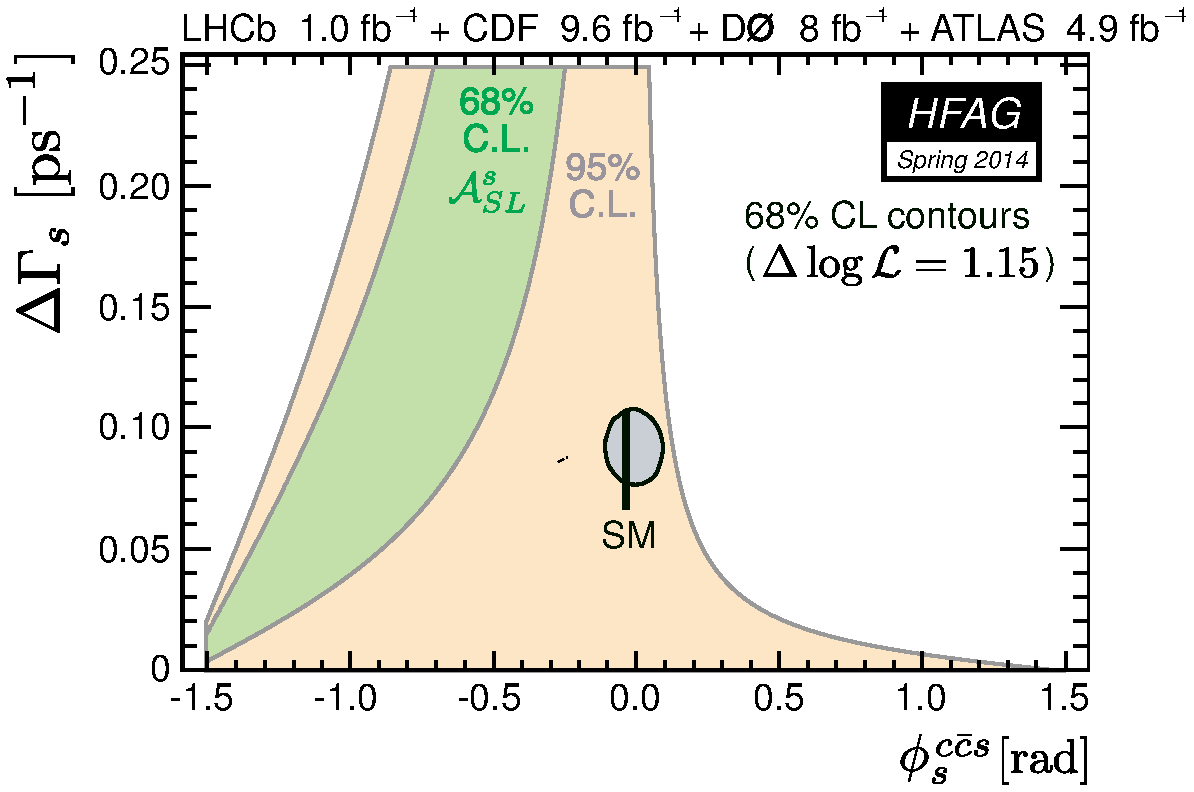
\includegraphics[width=0.8\textwidth]{graphics/pheno/hfag_spr2014_DGsphis_asls-crop-cmyk}
  \caption{Constraints in the $\phis$--$\DGs$ plane from measurements of CP violation in mixing ($\afs$, here represented as
	   $\mathcal{A}_\text{SL}^\text{s}$) by HFAG~\cite{Amhis:2012bh}, under the assumptions mentioned in the text.
           Both the 68\% (green) and 95\% (orange) confidence-level contours are shown.
           The confidence-level (CL) contour from the combination of direct $\phis$ (here represented as $\phisccs$) and $\DGs$
           measurements is shown as the grey area (see also Figure~\ref{fig:phisDGs} on page~\pageref{fig:phisDGs}).
           The Standard Model prediction is represented by the black bar.}
  \label{fig:phisDGs_asls}
\end{figure}
